% -*- TeX-master: "sicp.tex" -*-
\section{Procedures and the Processes They Generate}
\label{sec:1.2}


We have now considered the elements of programming: We have used
primitive arithmetic operations, we have combined these operations, and
we have abstracted these composite operations by defining them as compound
procedures.  But that is not enough to enable us to say that we know
how to program.  Our situation is analogous to that of someone who has
learned the rules for how the pieces move in chess but knows nothing
of typical openings, tactics, or strategy.  Like the novice chess
player, we don't yet know the common patterns of usage in the domain.
We lack the knowledge of which moves are worth making (which
procedures are worth defining).  We lack the experience to predict the
consequences of making a move (executing a procedure).

The ability to visualize the consequences of the actions under
consideration is crucial to becoming an expert programmer, just as it
is in any synthetic, creative activity.  In becoming an expert
photographer, for example, one must learn how to look at a scene and
know how dark each region will appear on a print for each possible
choice of exposure and development conditions.  Only then can one
reason backward, planning framing, lighting, exposure, and development
to obtain the desired effects.  So it is with programming, where we
are planning the course of action to be taken by a process and where
we control the process by means of a program.  To become experts, we
must learn to visualize the processes generated by various types of
procedures.  Only after we have developed such a skill can we learn
to reliably construct programs that exhibit the desired behavior.

A procedure is a pattern for the \textit{local evolution} of a
computational process.  It specifies how each stage of the process is
built upon the previous stage.  We would like to be able to make
statements about the overall, or \textit{global}, behavior of a
process whose local evolution has been specified by a procedure.  This
is very difficult to do in general, but we can at least try to
describe some typical patterns of process evolution.

In this section we will examine some common ``shapes'' for processes
generated by simple procedures.  We will also investigate the
rates at which these processes consume the important computational
resources of time and space.  The procedures we will consider
are very simple.  Their role is like that played by test patterns in
photography: as oversimplified prototypical patterns, rather than
practical examples in their own right.

\subsection{Linear Recursion and Iteration}
\label{sec:1.2.1}

\begin{figure}
  \centering
  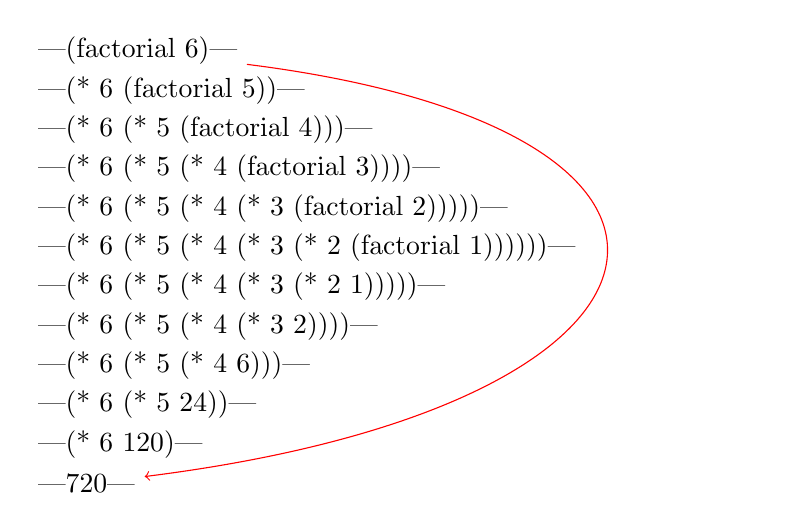
\begin{tikzpicture}
    [every node/.style={anchor=west}]
    \draw (0,0) node (a) {\scheme|(factorial 6)|} ;
    \draw (0,-0.5) node () {\scheme|(* 6 (factorial 5))|} ;
    \draw (0,-1) node () {\scheme|(* 6 (* 5 (factorial 4)))|} ;
    \draw (0,-1.5) node () {\scheme|(* 6 (* 5 (* 4 (factorial 3))))|} ;
    \draw (0,-2) node () {\scheme|(* 6 (* 5 (* 4 (* 3 (factorial 2)))))|} ;
    \draw (0,-2.5) node () {\scheme|(* 6 (* 5 (* 4 (* 3 (* 2 (factorial 1))))))|} ;
    \draw (0,-3) node () {\scheme|(* 6 (* 5 (* 4 (* 3 (* 2 1)))))|} ;
    \draw (0,-3.5) node () {\scheme|(* 6 (* 5 (* 4 (* 3 2))))|} ;
    \draw (0,-4) node () {\scheme|(* 6 (* 5 (* 4 6)))|} ;
    \draw (0,-4.5) node () {\scheme|(* 6 (* 5 24))|} ;
    \draw (0,-5) node () {\scheme|(* 6 120)|} ;
    \draw (0,-5.5) node (b) {\scheme|720|} ;
    \draw[->,red] (a) .. controls +(8cm,-1cm) and +(8cm,1cm) ..  (b) ;
  \end{tikzpicture}
  \caption{A linear recursive process for computing $6!$}
  \label{fig:1.3}
\end{figure}

We begin by considering the factorial function, defined by

\begin{displaymath}
n! = n \cdot (n-1) \cdot (n-2) \cdots 3 \cdot 2 \cdot 1
\end{displaymath}

There are many ways to compute factorials.  One way is to make use of
the observation that $n!$ is equal to $n$ times $(n - 1)!$ for
any positive integer $n$:


\begin{displaymath}
n! = n \cdot \left[ (n-1) \cdot (n-2) \cdots 3 \cdot 2 \cdot 1 \right] = n \cdot (n-1)!
\end{displaymath}

Thus, we can compute $n!$ by computing $(n - 1)!$ and multiplying the
result by $n$.  If we add the stipulation that $1!$ is equal to $1$,
this observation translates directly into a procedure:

\begin{schemedisplay}
(define (factorial n)
  (if (= n 1)
      1
      (* n (factorial (- n 1)))))
\end{schemedisplay}

We can use the substitution model of section \ref{sec:1.1.5} to watch
this procedure in action computing $6!$, as shown in figure
\ref{fig:1.3}.

Now let's take a different perspective on computing factorials.  We
could describe a rule for computing $n!$ by specifying that we first
multiply 1 by 2, then multiply the result by 3, then by 4, and so on
until we reach $n$.  More formally, we maintain a running product,
together with a counter that counts from 1 up to $n$.  We can describe
the computation by saying that the counter and the product
simultaneously change from one step to the next according to the rule

\begin{eqnarray}
  product &  \leftarrow & counter \cdot product \\
  counter  & \leftarrow &  counter  +  1
\end{eqnarray}


and stipulating that $n!$ is the value of the product when
the counter exceeds $n$.

\begin{equation}
  % TODO: Apply caption
  \frac{1}{1 / R_1 + 1 / R_2}
  %\caption{A linear iterative procedures for computing 6!}
  \label{fig:1.4}
\end{equation}

\begin{schemeregion}
Once again, we can recast our description as a procedure for computing
factorials:\footnote{In a real program we would probably use the block
  structure introduced in the last section to hide the definition of
  \scheme|fact-iter|:
\begin{schemedisplay}
(define (factorial n)
  (define (iter product counter)
    (if (> counter n)
        product
        (iter (* counter product)
              (+ counter 1))))
  (iter 1 1))
\end{schemedisplay}

We avoided doing this here so as to minimize the number of things to
think about at once.}
\end{schemeregion}

\begin{schemedisplay}
(define (factorial n)
  (fact-iter 1 1 n))

(define (fact-iter product counter max-count)
  (if (> counter max-count)
      product
      (fact-iter (* counter product)
                 (+ counter 1)
                 max-count)))
\end{schemedisplay}

As before, we can use the substitution model to visualize the process
of computing $6!$, as shown in figure \ref{fig:1.4}.

Compare the two processes.  From one point of view, they seem hardly
different at all.  Both compute the same mathematical function on the
same domain, and each requires a number of steps proportional to $n$
to compute $n!$.  Indeed, both processes even carry out the same
sequence of multiplications, obtaining the same sequence of partial
products.  On the other hand, when we consider the ``shapes'' of the
two processes, we find that they evolve quite differently.

Consider the first process.  The substitution model reveals a shape of
expansion followed by contraction, indicated by the arrow in figure
\ref{fig:1.3}.  The expansion occurs as the process builds up a chain
of \textit{deferred operations} (in this case, a chain of
multiplications).  The contraction occurs as the operations are
actually performed.  This type of process, characterized by a chain of
deferred operations, is called a \textit{recursive process}.  Carrying
out this process requires that the interpreter keep track of the
operations to be performed later on.  In the computation of
$n!$, the length of the chain of deferred multiplications, and
hence the amount of information needed to keep track of it, grows
linearly with $n$ (is proportional to $n$), just like
the number of steps.  Such a process is called a \textit{linear
  recursive process}.

By contrast, the second process does not grow and shrink.  At each
step, all we need to keep track of, for any $n$, are the current
values of the variables \scheme|product|, \scheme|counter|, and
\scheme|max-count|.  We call this an \textit{iterative process}.  In
general, an iterative process is one whose state can be summarized by
a fixed number of \textit{state variables}, together with a fixed rule
that describes how the state variables should be updated as the
process moves from state to state and an (optional) end test that
specifies conditions under which the process should terminate.  In
computing $n!$, the number of steps required grows linearly with $N$.
Such a process is called a \textit{linear iterative process}.

The contrast between the two processes can be seen in another way.  In
the iterative case, the program variables provide a complete
description of the state of the process at any point.  If we stopped
the computation between steps, all we would need to do to resume the
computation is to supply the interpreter with the values of the three
program variables.  Not so with the recursive process.  In this case
there is some additional ``hidden'' information, maintained by the
interpreter and not contained in the program variables, which
indicates ``where the process is'' in negotiating the chain of
deferred operations.  The longer the chain, the more information must
be maintained.\footnote{When we discuss the implementation of
  procedures on register machines in chapter \ref{chap:5}, we will see
  that any iterative process can be realized ``in hardware'' as a
  machine that has a fixed set of registers and no auxiliary memory.
  In contrast, realizing a recursive process requires a machine that
  uses an auxiliary data structure known as a \textit{stack}.}

In contrasting iteration and recursion, we must be careful not to
confuse the notion of a recursive \textit{process} with the notion of
a recursive \textit{procedure}.  When we describe a procedure as
recursive, we are referring to the syntactic fact that the procedure
definition refers (either directly or indirectly) to the procedure
itself.  But when we describe a process as following a pattern that
is, say, linearly recursive, we are speaking about how the process
evolves, not about the syntax of how a procedure is written.  It may
seem disturbing that we refer to a recursive procedure such as
\scheme|fact-iter| as generating an iterative process.  However, the
process really is iterative: Its state is captured completely by its
three state variables, and an interpreter need keep track of only
three variables in order to execute the process.

One reason that the distinction between process and procedure may be
confusing is that most implementations of common languages (including
Ada, Pascal, and C) are designed in such a way that the interpretation
of any recursive procedure consumes an amount of memory that grows
with the number of procedure calls, even when the process described
is, in principle, iterative.  As a consequence, these languages can
describe iterative processes only by resorting to special-purpose
``looping constructs'' such as \scheme|do|, \scheme|repeat|,
\scheme|until|, \scheme|for|, and \scheme|while|.  The implementation
of Scheme we shall consider in chapter 5 does not share this defect.
It will execute an iterative process in constant space, even if the
iterative process is described by a recursive procedure.  An
implementation with this property is called \textit{tail-recursive}.
With a tail-recursive implementation, iteration can be expressed using
the ordinary procedure call mechanism, so that special iteration
constructs are useful only as syntactic sugar.\footnote{Tail recursion
  has long been known as a compiler optimization trick.  A coherent
  semantic basis for tail recursion was provided by Carl Hewitt
  (1977), who explained it in terms of the ``message-passing'' model
  of computation that we shall discuss in chapter 3. Inspired by this,
  Gerald Jay Sussman and Guy Lewis Steele Jr. (see Steele 1975)
  constructed a tail-recursive interpreter for Scheme.  Steele later
  showed how tail recursion is a consequence of the natural way to
  compile procedure calls (Steele 1977).  The IEEE standard for Scheme
  requires that Scheme implementations be tail-recursive.}

\begin{Exercise}
\label{exc:1.9}
Each of the following two procedures defines a method for adding two
positive integers in terms of the procedures \scheme|inc|,
which increments its argument by 1, and \scheme|dec|, which decrements
its argument by 1.

\begin{schemedisplay}
(define (+ a b)
  (if (= a 0)
      b
      (inc (+ (dec a) b))))

(define (+ a b)
  (if (= a 0)
      b
      (+ (dec a) (inc b))))
\end{schemedisplay}

Using the substitution model, illustrate the process generated by each
procedure in evaluating \scheme|(+ 4 5)|.  Are these processes
iterative or recursive?
\end{Exercise}

\begin{Exercise}
\label{exc:1.10}
The following procedure computes a mathematical function called
Ackermann's function.

\begin{schemedisplay}
(define (A x y)
  (cond ((= y 0) 0)
        ((= x 0) (* 2 y))
        ((= y 1) 2)
        (else (A (- x 1)
                 (A x (- y 1))))))
\end{schemedisplay}
What are the values of the following expressions?

\begin{schemedisplay}
(A 1 10)

(A 2 4)

(A 3 3)
\end{schemedisplay}

Consider the following procedures, where \scheme|A| is the procedure  
defined above:
\begin{schemedisplay}
(define (f n) (A 0 n))

(define (g n) (A 1 n))

(define (h n) (A 2 n))

(define (k n) (* 5 n n))
\end{schemedisplay}

Give concise mathematical definitions for the functions computed by
the procedures \scheme|f|, \scheme|g|, and \scheme|h| for positive integer
values of $n$.  For example, \scheme|(k n)| computes $5n^2$
\end{Exercise}

\subsection{Tree Recursion}
\label{sec:1.2.2}



Another common pattern of computation is called \textit{tree
  recursion}.  As an example, consider computing the sequence of
Fibonacci numbers, in which each number is the sum of the preceding
two:

\begin{displaymath}
0, 1, 1, 2, 3, 5, 8, 13, 21, 34
\end{displaymath}

In general, the Fibonacci numbers can be defined by the rule
\begin{displaymath}
  {\rm Fib}(n) =
  \begin{cases}
    0 & {\rm if}~ n = 0 \\
    1 & {\rm if} n = 1 \\
    {\rm Fib}(n-1) + {\rm Fib}(n-2) & {\rm otherwise}
  \end{cases}
\end{displaymath}
We can immediately translate this definition into a recursive
procedure for computing Fibonacci numbers:

\begin{schemedisplay}
(define (fib n)
  (cond ((= n 0) 0)
        ((= n 1) 1)
        (else (+ (fib (- n 1))
                 (fib (- n 2))))))
\end{schemedisplay}

\begin{figure}
  % TODO: Add arrows to diagram (ch1-Z-G-13.gif)
\begin{tikzpicture}
    [level 1/.style={sibling distance=15em},
     level 2/.style={sibling distance=4em}]
    \node {fib 5}
      child { node {fib 4}
        child { node {fib 3} 
          child { node {fib 2}
            child { node {fib 1}
              child { node {1} } }
            child { node {fib 0} 
              child { node {0} } } }
          child { node {fib 1} 
            child { node {1} } } }
        child[missing] {}
        child { node {fib 2}
          child { node {fib 1}
            child { node {1} } }
          child { node {fib 0} 
            child { node {0} } } } }
      child { node {fib 3} 
        child { node {fib 2}
          child { node {fib 1}
            child { node {1} } }
          child { node {fib 0} 
            child { node {0} } } }
        child { node {fib 1} 
          child { node {1} } } } ;
\end{tikzpicture}
\caption{The tree-recursive proccess generated in computing (fib 5).}
\label{fig:1.5}
\end{figure}

Consider the pattern of this computation.  To compute \scheme|(fib 5)|,
we compute \scheme|(fib 4)| and \scheme|(fib 3)|.  To compute \scheme|(fib 4)|,
we compute \scheme|(fib 3)| and \scheme|(fib 2)|.  In general, the evolved
process looks like a tree, as shown in figure \ref{fig:1.5}.
Notice that the branches split into two at each level (except at the
bottom); this reflects the fact that the \scheme|fib| procedure calls
itself twice each time it is invoked.


This procedure is instructive as a prototypical tree recursion, but it
is a terrible way to compute Fibonacci numbers because it does so much
redundant computation.  Notice in figure \ref{fig:1.5} that the entire
computation of \scheme|(fib 3)| -- almost half the work -- is
duplicated.  In fact, it is not hard to show that the number of times
the procedure will compute \scheme|(fib 1)| or \scheme|(fib 0)| (the
number of leaves in the above tree, in general) is precisely ${\rm
  Fib}(n+1)$.  To get an idea of how bad this is, one can show that
the value of ${\rm Fib}(n)$ grows exponentially with $n$.  More
precisely (see exercise \ref{exc:1.13}), ${\rm Fib}(n)$ is the closest
% TODO: Verfy that these equations are in the right order.
integer to $\phi^n$, where $$\phi = \frac{1 + \sqrt 5}{2} \approx
1.6180$$ is the \textit{golden ratio}, which satisfies the
equation $$\phi^2 = \phi+1$$

Thus, the process uses a number of steps that grows exponentially with
the input.  On the other hand, the space required grows only linearly
with the input, because we need keep track only of which nodes are
above us in the tree at any point in the computation.  In general, the
number of steps required by a tree-recursive process will be
proportional to the number of nodes in the tree, while the space
required will be proportional to the maximum depth of the tree.

We can also formulate an iterative process for computing the
Fibonacci numbers.  The idea is to use a pair of integers $a$ and
$b$, initialized to  ${\rm Fib}(1) = 1$ and ${\rm Fib}(0) = 0$,
and to repeatedly apply the simultaneous
transformations
\begin{eqnarray*}
a & \leftarrow & a + b \\
b & \leftarrow & a
\end{eqnarray*}
It is not hard to show that, after applying this transformation $n$
times, $a$ and $b$ will be equal, respectively, to ${\rm Fib}(n+1)$
and ${\rm Fib}(n)$.  Thus, we can compute Fibonacci numbers
iteratively using the procedure

\begin{schemedisplay}
(define (fib n)
  (fib-iter 1 0 n))

(define (fib-iter a b count)
  (if (= count 0)
      b
      (fib-iter (+ a b) a (- count 1))))
\end{schemedisplay}

This second method for computing ${\rm Fib}(n)$ is a linear iteration.
The difference in number of steps required by the two methods -- one
linear in $n$, one growing as fast as ${\rm Fib}(n)$ itself -- is
enormous, even for small inputs.

One should not conclude from this that tree-recursive processes are
useless.  When we consider processes that operate on hierarchically
structured data rather than numbers, we will find that tree recursion
is a natural and powerful tool.\footnote{An example of this was hinted
  at in section \ref{sec:1.1.3}: The interpreter itself evaluates
  expressions using a tree-recursive process} But even in numerical
operations, tree-recursive processes can be useful in helping us to
understand and design programs.  For instance, although the first
\scheme|fib| procedure is much less efficient than the second one, it
is more straightforward, being little more than a translation into
Lisp of the definition of the Fibonacci sequence.  To formulate the
iterative algorithm required noticing that the computation could be
recast as an iteration with three state variables.

\subsubsection*{Example: Counting change}

It takes only a bit of cleverness to come up with the iterative
Fibonacci algorithm.  In contrast, consider the following problem: How
many different ways can we make change of \$1.00, given half-dollars,
quarters, dimes, nickels, and pennies?  More generally, can we write a
procedure to compute the number of ways to change any given amount of
money?

This problem has a simple solution as a recursive procedure.  Suppose
we think of the types of coins available as arranged in some order.
Then the following relation holds:

The number of ways to change amount $a$ using $n$ kinds of coins equals

\begin{itemize}
\item the number of ways to change amount $a$ using all but the first
  kind of coin, plus

\item the number of ways to change amount $a - d$ using all $n$ kinds
  of coins, where $d$ is the denomination of the first kind of coin.
\end{itemize}

To see why this is true, observe that the ways to make change can be
divided into two groups: those that do not use any of the first kind
of coin, and those that do.  Therefore, the total number of ways to
make change for some amount is equal to the number of ways to make
change for the amount without using any of the first kind of coin,
plus the number of ways to make change assuming that we do use the
first kind of coin.  But the latter number is equal to the number of
ways to make change for the amount that remains after using a coin of
the first kind.

Thus, we can recursively reduce the problem of changing a given amount
to the problem of changing smaller amounts using fewer kinds of coins.
Consider this reduction rule carefully, and convince yourself that we
can use it to describe an algorithm if we specify the following
degenerate cases:\footnote{For example, work through in detail how the
  reduction rule applies to the problem of making change for 10 cents
  using pennies and nickels.}

\begin{itemize}
\item If $a$ is exactly 0, we should count that as 1 way to make change.

\item If $a$ is less than 0, we should count that as 0 ways to make change.

\item If $n$ is 0, we should count that as 0 ways to make change.
\end{itemize}

We can easily translate this description into a recursive
procedure:

\begin{schemedisplay}
(define (count-change amount)
  (cc amount 5))
(define (cc amount kinds-of-coins)
  (cond ((= amount 0) 1)
        ((or (< amount 0) (= kinds-of-coins 0)) 0)
        (else (+ (cc amount
                     (- kinds-of-coins 1))
                 (cc (- amount
                        (first-denomination kinds-of-coins))
                     kinds-of-coins)))))
(define (first-denomination kinds-of-coins)
  (cond ((= kinds-of-coins 1) 1)
        ((= kinds-of-coins 2) 5)
        ((= kinds-of-coins 3) 10)
        ((= kinds-of-coins 4) 25)
        ((= kinds-of-coins 5) 50)))
\end{schemedisplay}
(The \scheme|first-denomination| procedure takes as input the number of
kinds of coins available and returns the denomination of the first
kind.  Here we are thinking of the coins as arranged in order from
largest to smallest, but any order would do as well.)  We can now
answer our original question about changing a dollar:

\begin{schemedisplay}
> (count-change 100)
292
\end{schemedisplay}

\scheme|Count-change| generates a tree-recursive process with
redundancies similar to those in our first implementation of
\scheme|fib|.  (It will take quite a while for that 292 to be
computed.)  On the other hand, it is not obvious how to design a
better algorithm for computing the result, and we leave this problem
as a challenge.  The observation that a tree-recursive process may be
highly inefficient but often easy to specify and understand has led
people to propose that one could get the best of both worlds by
designing a ``smart compiler'' that could transform tree-recursive
procedures into more efficient procedures that compute the same
result.\footnote{One approach to coping with redundant computations
  is to arrange matters so that we automatically construct a table of
  values as they are computed.  Each time we are asked to apply the
  procedure to some argument, we first look to see if the value is
  already stored in the table, in which case we avoid performing the
  redundant computation.  This strategy, known as \textit{tabulation}
  or \textit{memoization}, can be implemented in a straightforward
  way.  Tabulation can sometimes be used to transform processes that
  require an exponential number of steps (such as
  \scheme|count-change|) into processes whose space and time
  requirements grow linearly with the input.  See exercise
  \ref{exc:3.27}.}

\begin{Exercise}
\label{exc:1.11}
A function $f$ is defined by the rule that $f(n) = n {\rm ~if~} n < 3
{\rm ~and~} f(n) = f(n-1) + 2f(n-2) + 3f(n-3) {\rm ~if~} n \geq 3$.
Write a procedure that computes $f$ by means of a recursive process.
Write a procedure that computes $f$ by means of an iterative process.
\end{Exercise}

\begin{Exercise}
\label{exc:1.12}
The following pattern of numbers is called
\textit{Pascal's triangle}.

\begin{center}
\tt
\begin{tabular}{c}
  1 \\
  1 1 \\
  1 2 1 \\
1 3 3 1 \\
1 4 6 4 1
\end{tabular} 
\end{center}

The numbers at the edge of the triangle are all 1, and each number
inside the triangle is the sum of the two numbers above it.\footnote{
  The elements of Pascal's triangle are called the \textit{binomial
    coefficients}, because the \textit{n}th row consists of the
  coefficients of the terms in the expansion of $(x+y)^n$.  This
  pattern for computing the coefficients appeared in Blaise Pascal's
  1653 seminal work on probability theory, \textit{Trait\'e du
    triangle arithm\'etique}.  According to Knuth (1973), the same
  pattern appears in the \textit{Szu-yuen Y\"u-chien} (``The Precious
  Mirror of the Four Elements''), published by the Chinese
  mathematician Chu Shih-chieh in 1303, in the works of the
  twelfth-century Persian poet and mathematician Omar Khayyam, and in
  the works of the twelfth-century Hindu mathematician Bh\'ascara
  \'Ach\'arya.}

Write a procedure that computes elements of Pascal's triangle by means
of a recursive process.
\end{Exercise}

\begin{Exercise}
\label{exc:1.13}
Prove that ${\rm Fib}(n)$ is the closest integer to $\frac{\phi^n}{\sqrt 5}$,
where $\phi = \over{1 + \sqrt 5}{2}$  Hint: Let $\psi = \frac{1-\sqrt 5}{2}$.  Use
induction and the definition of the Fibonacci numbers (see
section \ref{sec:1.2.2}) to prove that ${\rm Fib}(n) = \frac{\phi^n - \psi^n}{\sqrt 5}$.
\end{Exercise}

\subsection{Orders of Growth}
\label{sec:1.2.3}

The previous examples illustrate that processes can differ
considerably in the rates at which they consume computational
resources.  One convenient way to describe this difference is to use
the notion of \textit{order of growth} to obtain a gross measure of the
resources required by a process as the inputs become larger.


Let $n$ be a parameter that measures the size of the problem, and let
$R(n)$ be the amount of resources the process requires for a problem
of size $n$.  In our previous examples we took $n$ to be the number
for which a given function is to be computed, but there are other
possibilities.  For instance, if our goal is to compute an
approximation to the square root of a number, we might take $n$ to be
the number of digits accuracy required.  For matrix multiplication we
might take $n$ to be the number of rows in the matrices.  In general
there are a number of properties of the problem with respect to which
it will be desirable to analyze a given process.  Similarly, $R(n)$
might measure the number of internal storage registers used, the
number of elementary machine operations performed, and so on.  In
computers that do only a fixed number of operations at a time, the
time required will be proportional to the number of elementary machine
operations performed.

We say that $R(n)$ has order of growth $\Theta(f(n))$ written $R(n) = \Theta(f(n))$) (pronounced ``theta of $f(n)$''), if there are
positive constants $k_1$ and $k_2$ independent of $n$ such that
$$k_1 f(n) \le R(N) \le k_2 f(n)$$
for any sufficiently large value of $n$.  (In other
words, for large $n$, the value $R(n)$) is sandwiched between $k_1f(n)$
and $k_2f(n)$.)

For instance, with the linear recursive process for computing
factorial described in section \ref{sec:1.2.1} the
number of steps grows proportionally to the input $n$.  Thus, the
steps required for this process grows as $\Theta(n)$.  We also saw
that the space required grows as $\Theta(n)$.  For the iterative
factorial, the number of steps is still $\Theta(n)$ but the space is
$\Theta(1)$ -- that is, constant.\footnote{These statements mask a
great deal of oversimplification.  For instance, if we count process
steps as ``machine operations'' we are making the assumption that the
number of machine operations needed to perform, say, a multiplication
is independent of the size of the numbers to be multiplied, which is
false if the numbers are sufficiently large.  Similar remarks hold for
the estimates of space.  Like the design and description of a process,
the analysis of a process can be carried out at various levels of
abstraction.} The tree-recursive Fibonacci computation requires
$\Theta(\phi^n)$ steps and space $\Theta(n)$, where $\phi$ is the
golden ratio described in section \ref{sec:1.2.2}.


Orders of growth provide only a crude description of the behavior of a
process.  For example, a process requiring $n^2$ steps and a process
requiring $1000n^2$ steps and a process requiring $3n^2 + 10n + 17$
steps all have $\Theta(n^2)$ order of growth.  On the other hand,
order of growth provides a useful indication of how we may expect the
behavior of the process to change as we change the size of the
problem.  For a $\Theta(n)$ (linear) process, doubling the size will
roughly double the amount of resources used.  For an exponential
process, each increment in problem size will multiply the resource
utilization by a constant factor.  In the remainder of section
\ref{sec:1.2} we will examine two algorithms whose order of growth is
logarithmic, so that doubling the problem size increases the resource
requirement by a constant amount.

\begin{Exercise}
\label{exc:1.14}
Draw the tree illustrating the process generated by the \scheme|count-change| procedure of section \ref{sec:1.2.2} in making
change for 11 cents.  What are the orders of growth of the space and
number of steps used by this process as the amount to be changed
increases?
\end{Exercise}

\begin{Exercise}
\label{exc:1.15}
The sine of an angle (specified in radians) can be computed by making
use of the approximation $\sin x \approx x$ if $x$ is sufficiently small, and the trigonometric
identity $$\sin r = 3 \sin \frac{r}{3} - 4 \sin^3 \frac{r}{3}$$
to reduce the size of the argument of $sin$.  (For purposes of
this exercise an angle is considered ``sufficiently small'' if its
magnitude is not greater than 0.1 radians.) These ideas are
incorporated in the following procedures:

\begin{schemedisplay}
(define (cube x) (* x x x))
(define (p x) (- (* 3 x) (* 4 (cube x))))
(define (sine angle)
   (if (not (> (abs angle) 0.1))
       angle
       (p (sine (/ angle 3.0)))))
\end{schemedisplay}
% TODO: use enumerate section
a.  How many times is the procedure \scheme|p| 
applied when \scheme|(sine 12.15)| is evaluated?

b.  What is the order of growth in space and number of steps (as a
function of $a$) used by the process generated by the \scheme|sine|
procedure when \scheme|(sine a)| is evaluated?
\end{Exercise}

\subsection{Exponentiation}
\label{sec:1.2.4}

Consider the problem of computing the exponential of a given number.
We would like a procedure that takes as arguments a base $b$ and a
positive integer exponent $n$ and computes $b^n$.  One way to do this
is via the recursive definition
\begin{eqnarray*}
b^n & = & b \cdot b^{n-1} \\
b^0 & = & 1 
\end{eqnarray*}
which translates readily into the procedure 

\begin{schemedisplay}
(define (expt b n)
  (if (= n 0)
      1
      (* b (expt b (- n 1)))))
\end{schemedisplay}
This is a linear recursive process, which requires $\Theta(n)$ steps
and $\Theta(n)$ space.  Just as with factorial, we can readily
formulate an equivalent linear iteration:

\begin{schemedisplay}
(define (expt b n)
  (expt-iter b n 1))

(define (expt-iter b counter product)
  (if (= counter 0)
      product
      (expt-iter b
                (- counter 1)
                (* b product)))) 
\end{schemedisplay}
This version requires $\Theta(n)$ steps and $\Theta(1)$ space.

We can compute exponentials in fewer steps by using successive
squaring.  For instance, rather than computing $b^8$ as
$$b \cdot (b \cdot (b \cdot (b \cdot (b \cdot (b \cdot (b \cdot b))))))$$
we can compute it using three multiplications:
\begin{eqnarray*}
b^2 & = & b \cdot b \\
b^4 & = & b^2 \cdot b^2 \\
b^8 & = & b^4 \cdot b^4 
\end{eqnarray*}

This method works fine for exponents that are powers of 2.  We can
also take advantage of successive squaring in computing exponentials
in general if we use the rule

\begin{displaymath}
  b^n =
  \begin{cases}
    \big(b^{b/2}\big)^2 & {\rm if~} n {\rm ~is~even} \\
    b \cdot b^{n-1} & {\rm if~} n {\rm ~is~odd}
  \end{cases}
\end{displaymath}
We can express this method as a procedure:


\begin{schemedisplay}
(define (fast-expt b n)
  (cond ((= n 0) 1)
        ((even? n) (square (fast-expt b (/ n 2))))
        (else (* b (fast-expt b (- n 1))))))
\end{schemedisplay}
where the predicate to test whether an integer is even is defined in terms of
the primitive procedure \scheme|remainder| by

\begin{schemedisplay}
(define (even? n)
  (= (remainder n 2) 0))
\end{schemedisplay}
The process evolved by \scheme|fast-expt| grows logarithmically with
$n$ in both space and number of steps.  To see this, observe that
computing $b^{2n}$ using \scheme|fast-expt| requires only one more
multiplication than computing $b^n$.  The size of the exponent we can
compute therefore doubles (approximately) with every new
multiplication we are allowed.  Thus, the number of multiplications
required for an exponent of $n$ grows about as fast as the logarithm
of $n$ to the base 2.  The process has $\Theta(\log n)$
growth.\footnote{More precisely, the number of multiplications
  required is equal to 1 less than the log base 2 of $n$ plus the
  number of ones in the binary representation of $n$.  This total is
  always less than twice the log base 2 of $n$.  The arbitrary
  constants $k_1$ and $k_2$ in the definition of order notation imply
  that, for a logarithmic process, the base to which logarithms are
  taken does not matter, so all such processes are described as
  $\Theta(\log n)$.}

The difference between $\Theta(\log n)$ growth and $\Theta(n)$ growth
becomes striking as $n$ becomes large.  For example,
\scheme|fast-expt| for $n = 1000$ requires only 14
multiplications.\footnote{You may wonder why anyone would care about
  raising numbers to the 1000th power.  See section \ref{sec:1.2.6}.}
It is also possible to use the idea of successive squaring to devise
an iterative algorithm that computes exponentials with a logarithmic
number of steps (see exercise \ref{exc:1.16}), although, as is often
the case with iterative algorithms, this is not written down so
straightforwardly as the recursive algorithm.\footnote{This iterative
  algorithm is ancient.  It appears in the \textit{Chandah-sutra} by
  \'Ach\'arya Pingala, written before 200 \textsc{b.c}.  See Knuth
  1981, section 4.6.3, for a full discussion and analysis of this and
  other methods of exponentiation.}



\begin{Exercise}
\label{exc:1.16}
Design a procedure that evolves an iterative exponentiation process
that uses successive squaring and uses a logarithmic number of steps,
as does \scheme|fast-expt|.  (Hint: Using the observation that
$(b^{n/2})^2 = (b^2)^{n/2}$, keep, along with the exponent $n$ and the
base $b$, an additional state variable $a$, and define the state
transformation in such a way that the product $a~b ^n$ is unchanged
from state to state.  At the beginning of the process $a$ is taken to
be 1, and the answer is given by the value of $a$ at the end of the
process.  In general, the technique of defining an \textit{invariant
  quantity} that remains unchanged from state to state is a powerful
way to think about the design of iterative algorithms.)
\end{Exercise}

\begin{Exercise}
\label{exc:1.17}
The exponentiation algorithms in this section are based on performing
exponentiation by means of repeated multiplication.  In a similar way,
one can perform integer multiplication by means of repeated addition.
The following multiplication procedure (in which it is assumed that
our language can only add, not multiply) is analogous to the \scheme|expt| procedure:

\begin{schemedisplay}
(define (* a b)
  (if (= b 0)
      0
      (+ a (* a (- b 1)))))
\end{schemedisplay}

This algorithm takes a number of steps that is linear in \scheme|b|.
Now suppose we include, together with addition, operations \scheme|double|,
which doubles an integer, and \scheme|halve|, which divides an (even)
integer by 2.  Using these, design a multiplication procedure analogous
to \scheme|fast-expt| that uses a logarithmic number of steps. 
\end{Exercise}

\begin{Exercise}
\label{exc:1.18}
Using the results of exercises \ref{exc:1.16} and \ref{exc:1.17},
devise a procedure that generates an iterative process for multiplying
two integers in terms of adding, doubling, and halving and uses a
logarithmic number of steps.\footnote{This algorithm, which is
  sometimes known as the ``Russian peasant method'' of multiplication,
  is ancient.  Examples of its use are found in the Rhind Papyrus, one
  of the two oldest mathematical documents in existence, written about
  1700 \textsc{b.c}. (and copied from an even older document) by an
  Egyptian scribe named A'h-mose.} 
\end{Exercise}

\begin{Exercise}
\label{exc:1.19}
There is a clever algorithm for computing the Fibonacci numbers in a
logarithmic number of steps.  Recall the transformation of the state
variables $a$ and $b$ in the \scheme|fib-iter| process of section
\ref{sec:1.2.2}: $a \leftarrow a + b$ and $b \leftarrow a$.  Call this
transformation $T$, and observe that applying $T$ over and over again
$n$ times, starting with 1 and 0, produces the pair ${\rm Fib}(n + 1)$
and ${\rm Fib}(n)$.  In other words, the Fibonacci numbers are produced by
applying $T^n$, the $n$th power of the transformation $T$, starting
with the pair $(1,0)$.  Now consider $T$ to be the special case of $p
= 0$ and $q = 1$ in a family of transformations $T_{pq}$, where
$T_{pq}$ transforms the pair $(a,b)$ according to $a \leftarrow bq +
aq + ap$ and $b \leftarrow bp + aq$.  Show that if we apply such a
transformation $T_{pq}$ twice, the effect is the same as using a
single transformation $T_{p'q'}$ of the same form, and compute $p'$
and $q'$ in terms of $p$ and $q$.  This gives us an explicit way to
square these transformations, and thus we can compute $T^n$ using
successive squaring, as in the \scheme|fast-expt| procedure.  Put this
all together to complete the following procedure, which runs in a
logarithmic number of steps:\footnote{This exercise was
suggested to us by Joe Stoy, based on an example in Kaldewaij 1990.}

\begin{schemedisplay}
(define (fib n)
  (fib-iter 1 0 0 1 n))
(define (fib-iter a b p q count)
  (cond ((= count 0) b)
        ((even? count)
         (fib-iter a
                   b
                   <??>      ; compute $p'$
                   <??>      ; compute $q'$
                   (/ count 2)))
        (else (fib-iter (+ (* b q) (* a q) (* a p))
                        (+ (* b p) (* a q))
                        p
                        q
                        (- count 1)))))
\end{schemedisplay}
\end{Exercise}

\subsection{Greatest Common Divisors}
\label{sec:1.2.5}

The greatest common divisor (GCD) of two integers $a$ and $b$ is
defined to be the largest integer that divides both $a$ and
$b$ with no remainder.  For example, the GCD of 16 and 28 is 4.  In chapter 2,
when we investigate how to implement rational-number arithmetic, we
will need to be able to compute GCDs in order to reduce
rational numbers to lowest terms.  (To reduce a rational number to
lowest terms, we must divide both the numerator and the denominator by their
GCD.  For example, 16/28 reduces to 4/7.)  One way to find the
GCD of two integers is to factor them and search for common
factors, but there is a famous algorithm that is much more efficient.

The idea of the algorithm is based on the observation that, if $r$ is
the remainder when $a$ is divided by $b$, then the common divisors of
$a$ and $b$ are precisely the same as the common divisors of $b$ and
$r$.  Thus, we can use the equation $${\rm GCD}(a,b) = {\rm GCD}(b,r)$$
to successively reduce the problem of computing a GCD to the
problem of computing the GCD of smaller and smaller pairs of
integers.  For example,
\begin{eqnarray*}
 {\rm GCD}(206,40) & = & {\rm GCD}(40,6) \\
 & = & {\rm GCD}(6,4) \\
 & = & {\rm GCD}(4,2) \\
 & = & {\rm GCD}(2,0) \\
 & = & 2
\end{eqnarray*}
reduces GCD(206,40) to GCD(2,0), which is 2.  It is possible to show
that starting with any two positive integers and performing repeated
reductions will always eventually produce a pair where the second
number is 0.  Then the GCD is the other number in the pair.  This
method for computing the GCD is known as \textit{Euclid's
  Algorithm}.\footnote{Euclid's Algorithm is so called because it
  appears in Euclid's $Elements$ (Book 7, ca. 300 \textsc{b.c}.).
  According to Knuth (1973), it can be considered the oldest known
  nontrivial algorithm.  The ancient Egyptian method of multiplication
  (exercise \ref{exc:1.18}) is surely older, but, as Knuth explains,
  Euclid's algorithm is the oldest known to have been presented as a
  general algorithm, rather than as a set of illustrative examples.}

It is easy to express Euclid's Algorithm as a procedure:
\begin{schemedisplay}
(define (gcd a b)
  (if (= b 0)
      a
      (gcd b (remainder a b))))
\end{schemedisplay}
This generates an iterative process, whose number of steps grows as
the logarithm of the numbers involved.

The fact that the number of steps required by Euclid's Algorithm has
logarithmic growth bears an interesting relation to the Fibonacci
numbers:

\begin{theorem}[Lam\'e's Theorem]
  If Euclid's Algorithm requires $k$ steps to compute the GCD of some
  pair, then the smaller number in the pair must be greater than or
  equal to the $k$th Fibonacci number.\footnote{This theorem was
    proved in 1845 by Gabriel Lam\'e, a French mathematician and
    engineer known chiefly for his contributions to mathematical
    physics.  To prove the theorem, we consider pairs $(a_{k}
    ,b_{k})$, where $a_k \ge b_k$, for which Euclid's Algorithm
    terminates in $k$ steps.  The proof is based on the claim that, if
    $(a_{k+1}, b_{k+1}) \mapsto (a_k, b_k) \mapsto (a_{k-1},
    b_{k-1})$ are three successive pairs in the reduction process,
    then we must have $b_{k+1} \ge b_k + b_{k-1}$.  To verify the
    claim, consider that a reduction step is defined by applying the
    transformation $a_{k-1} = b_k$, $b_{k-1} = {\rm remainder~of~} a_k
    {\rm ~divided~by~} b_k$.  The second equation means that $a_k =
    qb_k + b_{k-1}$ for some positive integer $q$.  And since $q$ must
    be at least 1 we have $a_k = qb_k + b_{k-1} \ge b_k + b_{k-1}$.
    But in the previous reduction step we have $b_{k+1} = a_k$.
    Therefore, $b_{k+1} = a_k \ge b_k + b_{k-1}$.  This verifies the
    claim.  Now we can prove the theorem by induction on $k$, the
    number of steps that the algorithm requires to terminate.  The
    result is true for $k = 1$, since this merely requires that $b$ be
    at least as large as ${\rm Fib}(1) = 1$.  Now, assume that the
    result is true for all integers less than or equal to $k$ and
    establish the result for $k + 1$.  Let $(a_{k+1}, b_{k+1})
    \mapsto (a_k, b_k) \mapsto (a_{k-1}, b_{k-1})$ be
    successive pairs in the reduction process.  By our induction
    hypotheses, we have $b_{k-1} \ge {\rm Fib}(k - 1)$ and $b_k \ge
    {\rm Fib}(k)$.  Thus, applying the claim we just proved together
    with the definition of the Fibonacci numbers gives $b_{k+1} \ge
    b_k + b_{k-1} \ge {\rm Fib}(k) + {\rm Fib}(k - 1) = {\rm
      Fib}(k+1)$, which completes the proof of Lam\'e's Theorem.}
\end{theorem}



We can use this theorem to get an order-of-growth estimate for Euclid's
Algorithm.  Let $n$ be the smaller of the two inputs to the
procedure.  If the process takes $k$ steps, then we must have 
$n \ge {\rm Fib}(k) \approx \frac{\phi^k}{\sqrt 5}$.  Therefore
the number of steps $k$ grows as the logarithm (to the base
$\phi$) of $n$.  Hence, the order of growth is $\Theta(\log n)$.

\begin{Exercise}
\label{exc:1.20}
The process that a procedure generates is of course dependent on the
rules used by the interpreter.  As an example, consider the iterative
\scheme|gcd| procedure given above.  Suppose we were to interpret this
procedure using normal-order evaluation, as discussed in section
\ref{sec:1.1.5}.  (The normal-order-evaluation rule for \scheme|if| is
described in exercise \ref{exc:1.5}.)  Using the substitution method
(for normal order), illustrate the process generated in evaluating
\scheme|(gcd 206 40)| and indicate the \scheme|remainder| operations
that are actually performed.  How many \scheme|remainder| operations
are actually performed in the normal-order evaluation of \scheme|(gcd
206 40)|?  In the applicative-order evaluation?
\end{Exercise}

\subsection{Example: Testing for Primality}
\label{sec:1.2.6}



This section describes two methods for checking the primality of an
integer $n$, one with order of growth $\Theta(\sqrt n)$, and a
``probabilistic'' algorithm with order of growth $\Theta(\log n)$.
The exercises at the end of this section suggest programming projects
based on these algorithms.

\subsubsection*{Searching for divisors}

Since ancient times, mathematicians have been fascinated by problems
concerning prime numbers, and many people have worked on the problem
of determining ways to test if numbers are prime.  One way
to test if a number is prime is to find the number's divisors.  The
following program finds the smallest integral divisor (greater than 1)
of a given number $n$.  It does this in a straightforward way, by
testing $n$ for divisibility by successive integers starting with 2.

\begin{schemedisplay}
(define (smallest-divisor n)
  (find-divisor n 2))
(define (find-divisor n test-divisor)
  (cond ((> (square test-divisor) n) n)
        ((divides? test-divisor n) test-divisor)
        (else (find-divisor n (+ test-divisor 1)))))
(define (divides? a b)
  (= (remainder b a) 0))
\end{schemedisplay}

We can test whether a number is prime as follows: $n$ is prime if
and only if $n$ is its own smallest divisor.

\begin{schemedisplay}
(define (prime? n)
  (= n (smallest-divisor n)))
\end{schemedisplay}

The end test for \scheme|find-divisor| is based on the fact that if
$n$ is not prime it must have a divisor less than or equal to $\sqrt
n$.\footnote{If $d$ is a divisor of $n$, then so is $n/d$.  But $d$
  and $n/d$ cannot both be greater than $\sqrt n$} This means that the
algorithm need only test divisors between 1 and $\sqrt n$.
Consequently, the number of steps required to identify $n$ as prime
will have order of growth $\Theta(\sqrt n)$.

\subsubsection*{The Fermat test}

The $\Theta(\log n)$ primality test is based on a result from number
theory known as Fermat's Little Theorem.\footnote{Pierre de Fermat
  (1601-1665) is considered to be the founder of modern number theory.
  He obtained many important number-theoretic results, but he usually
  announced just the results, without providing his proofs.  Fermat's
  Little Theorem was stated in a letter he wrote in 1640.  The first
  published proof was given by Euler in 1736 (and an earlier,
  identical proof was discovered in the unpublished manuscripts of
  Leibniz).  The most famous of Fermat's results -- known as Fermat's
  Last Theorem -- was jotted down in 1637 in his copy of the book
  \textit{Arithmetic} (by the third-century Greek mathematician
  Diophantus) with the remark ``I have discovered a truly remarkable
  proof, but this margin is too small to contain it.''  Finding a
  proof of Fermat's Last Theorem became one of the most famous
  challenges in number theory.  A complete solution was finally given
  in 1995 by Andrew Wiles of Princeton University.  }

\begin{theorem}[Fermat's Little Theorem]
  If $n$ is a prime number and $a$ is any positive integer less than
  $n$, then $a$ raised to the $n$th power is congruent to $a$ modulo
  $n$.
\end{theorem}

(Two numbers are said to be \textit{congruent modulo} $n$ if
they both have the same remainder when divided by $n$.  The
remainder of a number $a$ when divided by $n$ is also referred to as
the \textit{remainder of} $a$ \textit{modulo} $n$, or simply as $a$ 
\textit{modulo} $n$.)

If $n$ is not prime, then, in general, most of the numbers $a < n$ will not
satisfy the above relation.  This leads to the following algorithm for
testing primality: Given a number $n$, pick a random number $a < n$ and
compute the remainder of $a^n$ modulo $n$.  If the result is not equal to
$a$, then $n$ is certainly not prime.  If it is $a$, then chances are good
that $n$ is prime.  Now pick another random number $a$ and test it with the
same method.  If it also satisfies the equation, then we can be even more
confident that $n$ is prime.  By trying more and more values of $a$, we can
increase our confidence in the result.  This algorithm is known as the
Fermat test.

To implement the Fermat test, we need a procedure that computes the
exponential of a number modulo another number:

\begin{schemedisplay}
(define (expmod base exp m)
  (cond ((= exp 0) 1)
        ((even? exp)
         (remainder (square (expmod base (/ exp 2) m))
                    m))
        (else
         (remainder (* base (expmod base (- exp 1) m))
                    m))))        
\end{schemedisplay}
This is very similar to the \scheme|fast-expt| procedure of section
\ref{sec:1.2.4}.  It uses successive squaring, so that the number of
steps grows logarithmically with the exponent.\footnote{The reduction
  steps in the cases where the exponent $e$ is greater than 1
  are based on the fact that, for any integers $x$, $y$,
  and $m$, we can find the remainder of $x$ times
  $y$ modulo $m$ by computing separately the remainders
  of $x$ modulo $m$ and $y$ modulo $m$,
  multiplying these, and then taking the remainder of the result
  modulo $m$.  For instance, in the case where $e$ is
  even, we compute the remainder of $b^{e/2}$
  modulo $m$, square this, and take the remainder modulo
  $m$.  This technique is useful because it means we can
  perform our computation without ever having to deal with numbers
  much larger than $m$.  (Compare exercise \ref{exc:1.25})}

The Fermat test is performed by choosing at random a number $a$
between $1$ and $n - 1$ inclusive and checking whether the remainder
modulo $n$ of the $n$th power of $a$ is equal to $a$.  The random
number $a$ is chosen using the procedure \scheme|random|, which we assume is
included as a primitive in Scheme. \scheme|Random| returns a
nonnegative integer less than its integer input.  Hence, to obtain a random
number between $1$ and $n - 1$, we call \scheme|random| with an input of
$n - 1$ and add 1 to the result:

\begin{schemedisplay}
(define (fermat-test n)
  (define (try-it a)
    (= (expmod a n n) a))
  (try-it (+ 1 (random (- n 1)))))
\end{schemedisplay}

The following procedure runs the test a given number of times, as
specified by a parameter.  Its value is true if the test succeeds
every time, and false otherwise.

\begin{schemedisplay}
(define (fast-prime? n times)
  (cond ((= times 0) true)
        ((fermat-test n) (fast-prime? n (- times 1)))
        (else false)))
\end{schemedisplay}

\subsubsection*{Probabilistic methods}

The Fermat test differs in character from most familiar algorithms, in
which one computes an answer that is guaranteed to be correct.  Here,
the answer obtained is only probably correct.  More precisely, if $n$
ever fails the Fermat test, we can be certain that $n$ is not prime.
But the fact that $n$ passes the test, while an extremely strong
indication, is still not a guarantee that $n$ is prime.  What we would
like to say is that for any number $n$, if we perform the test enough
times and find that $n$ always passes the test, then the probability
of error in our primality test can be made as small as we like.

Unfortunately, this assertion is not quite correct.  There do exist
numbers that fool the Fermat test: numbers $n$ that are not prime and
yet have the property that $a^n$ is congruent to $a$ modulo $n$ for
all integers $a < n$.  Such numbers are extremely rare, so the Fermat
test is quite reliable in practice.\footnote{\label{fn:1.47}Numbers
  that fool the Fermat test are called \textit{Carmichael numbers},
  and little is known about them other than that they are extremely
  rare.  There are 255 Carmichael numbers below 100,000,000.  The
  smallest few are 561, 1105, 1729, 2465, 2821, and 6601.  In testing
  primality of very large numbers chosen at random, the chance of
  stumbling upon a value that fools the Fermat test is less than the
  chance that cosmic radiation will cause the computer to make an
  error in carrying out a ``correct'' algorithm.  Considering an
  algorithm to be inadequate for the first reason but not for the
  second illustrates the difference between mathematics and
  engineering.}  There are variations of the Fermat test that cannot
be fooled.  In these tests, as with the Fermat method, one tests the
primality of an integer $n$ by choosing a random integer $a < n$ and
checking some condition that depends upon $n$ and $a$.  (See exercise
\ref{exc:1.28} for an example of such a test.)  On the other hand, in
contrast to the Fermat test, one can prove that, for any $n$, the
condition does not hold for most of the integers $a < n$ unless $n$ is
prime.  Thus, if $n$ passes the test for some random choice of $a$,
the chances are better than even that $n$ is prime.  If $n$ passes the
test for two random choices of $a$, the chances are better than 3 out
of 4 that $n$ is prime. By running the test with more and more
randomly chosen values of $a$ we can make the probability of error as
small as we like.

The existence of tests for which one can prove that the chance of
error becomes arbitrarily small has sparked interest in algorithms of
this type, which have come to be known as \idef{probabilistic
  algorithms}.  There is a great deal of research activity in this
area, and probabilistic algorithms have been fruitfully applied to
many fields.\footnote{One of the most striking applications of
  probabilistic prime testing has been to the field of cryptography.
  Although it is now computationally infeasible to factor an arbitrary
  200-digit number, the primality of such a number can be checked in a
  few seconds with the Fermat test.  This fact forms the basis of a
  technique for constructing ``unbreakable codes'' suggested by
  Rivest, Shamir, and Adleman (1977).  The resulting \textit{RSA
    algorithm} has become a widely used technique for enhancing the
  security of electronic communications.  Because of this and related
  developments, the study of prime numbers, once considered the
  epitome of a topic in ``pure'' mathematics to be studied only for
  its own sake, now turns out to have important practical applications
  to cryptography, electronic funds transfer, and information
  retrieval.}

\begin{Exercise}
\label{exc:1.21}
Use the \scheme|smallest-divisor| procedure to find the smallest divisor
of each of the following numbers: 199, 1999, 19999.
\end{Exercise}

\begin{Exercise}
\label{exc:1.22}
Most Lisp implementations include a primitive called \scheme|runtime|
that returns an integer that specifies the amount of time the system
has been running (measured, for example, in microseconds).  The
following \scheme|timed-prime-test| procedure, when called with an
integer $n$, prints $n$ and checks to see if $n$ is prime.  If $n$ is
prime, the procedure prints three asterisks followed by the amount of time
used in performing the test.

\begin{schemedisplay}
(define (timed-prime-test n)
  (newline)
  (display n)
  (start-prime-test n (runtime)))
(define (start-prime-test n start-time)
  (if (prime? n)
      (report-prime (- (runtime) start-time))))
(define (report-prime elapsed-time)
  (display " *** ")
  (display elapsed-time))
\end{schemedisplay}
Using this procedure, write a procedure \scheme|search-for-primes| that
checks the primality of consecutive odd integers in a specified range.
Use your procedure to find the three smallest primes larger than 1000;
larger than 10,000; larger than 100,000; larger than 1,000,000.  Note
the time needed to test each prime.  Since the testing algorithm has
order of growth of $\Theta(\sqrt n)$, you should expect that testing
for primes around 10,000 should take about $\sqrt( 10$ times as long
as testing for primes around 1000.  Do your timing data bear this out?
How well do the data for 100,000 and 1,000,000 support the $\sqrt n$
prediction?  Is your result compatible with the notion that programs
on your machine run in time proportional to the number of steps
required for the computation?
\end{Exercise}

\begin{Exercise}
\label{exc:1.23}
The \scheme|smallest-divisor| procedure shown at the start of this section
does lots of needless testing: After it checks to see if the
number is divisible by 2 there is no point in checking to see if
it is divisible by any larger even numbers.  This suggests that the
values used for \scheme|test-divisor| should not be 2, 3, 4, 5, 6,
\scheme|...|, but rather 2, 3, 5, 7, 9, \scheme|...|.  To implement this
change, define a procedure \scheme|next| that returns 3 if its input is
equal to 2 and otherwise returns its input plus 2.  Modify the \scheme|smallest-divisor| procedure to use \scheme|(next test-divisor)| instead
of \scheme|(+ test-divisor 1)|.  With \scheme|timed-prime-test|
incorporating this modified version of \scheme|smallest-divisor|, run the
test for each of the 12 primes found in
exercise \ref{exc:1.22}.  Since this modification halves the
number of test steps, you should expect it to run about twice as fast.
Is this expectation confirmed?  If not, what is the observed ratio of
the speeds of the two algorithms, and how do you explain the fact that
it is different from 2?
\end{Exercise}

\begin{Exercise}
\label{exc:1.24}
Modify the \scheme|timed-prime-test| procedure of
exercise \ref{exc:1.22} to use \scheme|fast-prime?| (the
Fermat method), and test each of the 12 primes you found in that
exercise.  Since the Fermat test has $\Theta(\log n)$ growth, how
would you expect the time to test primes near 1,000,000 to compare
with the time needed to test primes near 1000?  Do your data bear this
out?  Can you explain any discrepancy you find?
\end{Exercise}


\begin{Exercise}
\label{exc:1.25}
 Alyssa P. Hacker complains that we went to a lot of extra work in
writing \scheme|expmod|.  After all, she says, since we already know how
to compute exponentials, we could have simply written

\begin{schemedisplay}
(define (expmod base exp m)
  (remainder (fast-expt base exp) m))
\end{schemedisplay}
Is she correct?  Would this procedure serve as well for our fast prime
tester?  Explain.
\end{Exercise}


\begin{Exercise}
\label{exc:1.26}
Louis Reasoner is having great difficulty doing exercise
\ref{exc:1.24}.  His \scheme|fast-prime?| test seems to run more
slowly than his \scheme|prime?| test.  Louis calls his friend Eva Lu
Ator over to help.  When they examine Louis's code, they find that he
has rewritten the \scheme|expmod| procedure to use an explicit
multiplication, rather than calling \scheme|square|:

\begin{schemedisplay}
(define (expmod base exp m)
  (cond ((= exp 0) 1)
        ((even? exp)
         (remainder (* (expmod base (/ exp 2) m)
                       (expmod base (/ exp 2) m))
                    m))
        (else
         (remainder (* base (expmod base (- exp 1) m))
                    m))))
\end{schemedisplay}
``I don't see what difference that could make,'' says Louis.  ``I
do.''  says Eva.  ``By writing the procedure like that, you have
transformed the $\Theta(\log n)$ process into a $\Theta(n)$ process.''
Explain.
\end{Exercise}

\begin{Exercise}
\label{exc:1.27}
Demonstrate that the Carmichael numbers listed in footnote \ref{fn:1.47}
really do fool the Fermat test.  That is, write a procedure that takes
an integer $n$ and tests whether $a^n$ is congruent to $a$ modulo $n$
for every $a < n$, and try your procedure on the given Carmichael
numbers.
\end{Exercise}

\begin{Exercise}
\label{exc:1.28}
One variant of the Fermat test that cannot be fooled is called the
\textit{Miller-Rabin test} (Miller 1976; Rabin 1980).  This starts from
an alternate form of Fermat's Little Theorem, which states that if $n$
is a prime number and $a$ is any positive integer less than $n$, then
$a$ raised to the $n - 1$)st power is congruent to $1$ modulo $n$.  To test
the primality of a number $n$ by the Miller-Rabin test, we pick a
random number $a < n$ and raise $a$ to the $(n - 1)$st power modulo $n$
using the \scheme|expmod| procedure.  However, whenever we perform the
squaring step in \scheme|expmod|, we check to see if we have discovered a
``nontrivial square root of 1 modulo $n$,'' that is, a number not
equal to $1$ or $n - 1$ whose square is equal to 1 modulo $n$.  It is
possible to prove that if such a nontrivial square root of 1 exists,
then $n$ is not prime.  It is also possible to prove that if $n$ is an
odd number that is not prime, then, for at least half the numbers
$a < n$, computing $a^{n-1}$ in this way will reveal a nontrivial
square root of 1 modulo $n$.  (This is why the Miller-Rabin test
cannot be fooled.)  Modify the \scheme|expmod| procedure to signal if it
discovers a nontrivial square root of 1, and use this to implement
the Miller-Rabin test with a procedure analogous to \scheme|fermat-test|.
Check your procedure by testing various known primes and non-primes.
Hint: One convenient way to make \scheme|expmod| signal is to have it
return 0.
\end{Exercise}